% $Id: template.tex 11 2007-04-03 22:25:53Z jpeltier $

%\documentclass{vgtc}                          % final (conference style)
\documentclass[review]{vgtc}                 % review
%\documentclass[widereview]{vgtc}             % wide-spaced review
%\documentclass[preprint]{vgtc}               % preprint
%\documentclass[electronic]{vgtc}             % electronic version

%% Uncomment one of the lines above depending on where your paper is
%% in the conference process. ``review'' and ``widereview'' are for review
%% submission, ``preprint'' is for pre-publication, and the final version
%% doesn't use a specific qualifier. Further, ``electronic'' includes
%% hyperreferences for more convenient online viewing.

%% Please use one of the ``review'' options in combination with the
%% assigned online id (see below) ONLY if your paper uses a double blind
%% review process. Some conferences, like IEEE Vis and InfoVis, have NOT
%% in the past.

%% Figures should be in CMYK or Grey scale format, otherwise, colour 
%% shifting may occur during the printing process.

%% These three lines bring in essential packages: ``mathptmx'' for Type 1 
%% typefaces, ``graphicx'' for inclusion of EPS figures. and ``times''
%% for proper handling of the times font family.

\usepackage{mathptmx}
\usepackage{graphicx}
\usepackage{times}
\usepackage{subfigure}
\usepackage{flushend}

%% We encourage the use of mathptmx for consistent usage of times font
%% throughout the proceedings. However, if you encounter conflicts
%% with other math-related packages, you may want to disable it.

%% If you are submitting a paper to a conference for review with a double
%% blind reviewing process, please replace the value ``0'' below with your
%% OnlineID. Otherwise, you may safely leave it at ``0''.
\onlineid{114}

%% declare the category of your paper, only shown in review mode
\vgtccategory{System}

%% allow for this line if you want the electronic option to work properly
\vgtcinsertpkg

%% In preprint mode you may define your own headline.
%\preprinttext{To appear in an IEEE VGTC sponsored conference.}

%% Paper title.

\renewcommand{\fboxsep}{0pt}

%Guiding DBS Interventions by ...
\title{Guiding Deep Brain Stimulation Interventions \\ by Fusing Multimodal Uncertainty Regions}
%\title{Supporting Deep Brain Stimulation Interventions \\ by Fusing Microelectrode Recordings with Imaging Data}

\author{Alexander Bock\thanks{alexander.bock@liu.se} \\ %
%	\parbox{1in}{\scriptsize \centering Scientific Visualization Group \\ 	Link\"oping University}
	\parbox{1in}{\scriptsize \centering Link\"oping University}
\and Norbert Lang\thanks{nlang@barbaraklinik.de} \\ %
	\parbox{1in}{\scriptsize \centering St. Barbara Hospital \\ Hamm}
\and Gianpaolo Evangelista\thanks{giaev@itn.liu.se} \\ %
	\parbox{1in}{\scriptsize \centering Link\"oping University}
%	\parbox{1in}{\scriptsize \centering Sound Processing Group \\ Link\"oping University}
\and Ralph Lehrke\thanks{rlehrke@barbaraklinik.de} \\ %
	\parbox{1in}{\scriptsize \centering St. Barbara Hospital \\ Hamm}
\and Timo Ropinski\thanks{timo.ropinski@liu.se} \\ %
	\parbox{1in}{\scriptsize \centering Link\"oping University}
%	\parbox{1in}{\scriptsize \centering Scientific Visualization Group \\ 	Link\"oping University}
}

\shortauthortitle{Bock \MakeLowercase{\textit{et al.}}: DBS Visualization}

%% Abstract section.
\abstract{Deep Brain Stimulation (DBS) is a surgical intervention that is known to reduce or eliminate the symptoms of common movement disorders, such as the Parkinson's disease, dystonia, or tremor. During the intervention the surgeon places electrodes within the patient's brain so that specific regions are stimulated. Since these regions span only a couple of millimeters and electrode misplacement has severe consequences, reliable and accurate navigation is of great importance. Usually the surgeon relies on fused CT and MRI data sets, as well as direct feedback from the patient. More recently Microelectrode Recordings (MER), which support navigation by measuring the electric field of the patient's brain, are also facilitated. We propose a visualization system that fuses the different modalities, i.\,e., imaging data, MER and patient checks, in an intuitive way to present placement-related information in a consistent view with the goal of supporting the surgeon in the final placement of the stimulating electrode. We will describe the design considerations for our system, the technical realization, the outcome of the proposed system, and an evaluation.
}
%While MER has the potential to improve placement accuracy, the fusion with the available imaging data is performed by the surgeon through mental registration, which results in a higher cognitive load and potentially affects efficiency.

%% ACM Computing Classification System (CCS). 
%% See <http://www.acm.org/class/1998/> for details.
%% The ``\CCScat'' command takes four arguments.

%\keywords{Deep brain stimulation, multimodal visualization, multiple views.}

\CCScatlist{ 
  \CCScat{I.3.7 }{Three-Dimensional Graphics and Realism}{}
}

%% Copyright space is enabled by default as required by guidelines.
%% It is disabled by the 'review' option or via the following command:
% \nocopyrightspace

%%%%%%%%%%%%%%%%%%%%%%%%%%%%%%%%%%%%%%%%%%%%%%%%%%%%%%%%%%%%%%%%
%%%%%%%%%%%%%%%%%%%%%% START OF THE PAPER %%%%%%%%%%%%%%%%%%%%%%
%%%%%%%%%%%%%%%%%%%%%%%%%%%%%%%%%%%%%%%%%%%%%%%%%%%%%%%%%%%%%%%%%

\begin{document}
\firstsection{Introduction}\label{sec:introduction}

\maketitle

Due to the advances in medicine, society is now facing the problems of an aging population suffering an increasing amount of age-related diseases. One such group of frequently occurring age-related diseases are \emph{movement disorders}, such as Parkinson's Disease (PD), dystonia, or tremors that greatly affect the patients' quality of life. As both symptoms regarding motor skills as well as psychological consequences of these diseases have a great impact on everyday life, successful treatment strategies are of increasing importance.

Deep Brain Stimulation (DBS) is a well-established procedure for reducing the symptoms of these diseases~\cite{Lindberg2002,Benabid2009} and improving the overall quality of life in the cases where medication is not a viable option. To conduct a DBS, electrodes are implanted into specific regions of the brain, which then emit electrical signals to stimulate these regions. In the case of PD the most effective target areas for electrode placement are the subthalamic nuclei (STN) that reach sizes of a few millimeters~\cite{Richter2004} and are located in both hemispheres. As misplaced stimulation electrodes can have severe side effects, such as speech difficulties, increased tremor, or long term memory problems~\cite{Astrom2010}, accurate electrode placement is crucial~\cite{Rodriguez-Oroz2005}. Nowadays, the access path to the target region is planned using magnetic resonance imaging (MRI). However, besides the low signal-to-noise ratio, a major downside of this imaging modality is that the STN might not be visible in every patient~\cite{Starr2002}. Therefore, surgeons often use an atlas-based approach to locate the STN within the MRI data, which is prone to registration errors, is not patient specific, and lacks visual assessment. To further verify the electrode placement the patient performs simple tasks during the operation, which are monitored by the surgical staff and are used to localize the electrodes position. Depending on the location of the electrode, a different region of the brain is stimulated, manifesting in measurable responses from the patient. These responses can be of cognitive, e.\,g.,~memory impairment, or motorical, e.\,g.,~increased tremor or spech impariment, nature. To further reduce the uncertainty of the electrode placement intra-operative x-ray scans can be performed to confirm the electrode placement.
%
% Depending on the electrodes location along the access path either temporary memory-loss, speech problems or a tremor increase can occur.
%
%In addition to the increased precision and in contrast to x-ray scanning, this method does not use any ionizing radiation which should be, especially in the brain, avoided at all costs. While x-ray scans might still be performed after the surgery as a final check, MER has the potential to reduce the need for intra-operative scans. Only by combining MER data with the structural information acquired through MRI, the neurosurgeon is able to plan and perform all necessary steps during the DBS intervention. Furthermore, intra-operative patient checks do also not become obsolete, as their results allow to draw direct conclusions about the influence of the placed electrode. 
%
In recent years, Microelectrode Recording (MER) has emerged as an additional technique allowing the surgeon to better locate the target region for DBS intra-operatively~\cite{Lenz1988}. MER measures the electrical field of the brain during the surgery by inserting electrodes into the access path. The measured information is presented to the surgical staff by showing the amplitude in the time domain for each electrode, from which the expert differentiates functional regions of the brain. In order to allow for an intuitive and accurate placement of the electrodes, it is important that the surgeon has access to all these modalities in a unified manner.

Within this paper we propose an interactive visualization system to support the DBS placement procedure by combining the values and uncertainties of these different measurements, whereby the combined information is used to guide the surgeon to the optimal placement location. To this end, we provide two views enhancing the final placement of the electrode. These views combine the information about the target region gathered from different sources, i.\,e. pre-operative scans, x-ray scans, MER, patient checks, and present them to the surgeon. One of the views fuses this data with the structural information surrounding the intended target region in a multimodal visualization. This enables a mental registration of the measured data to the imaging modalities and, thereby, provides context that the surgeon can draw upon during the placement decision. The other provides an information visualization approach to present the data in a quantitative way.

In the remainder of this paper we will briefly explain the DBS process, derive uncertainty regions for the measurements, and show how to visualize them in a unified approach.

%
% This is beneficial, as it has been shown in other contexts, since presenting multiple modalities in an integrated manner can improve the information gathering process~\cite{10.1109/BIOMEDVIS.1995.10008}. 
%By visually overlapping the potential target areas, the surgeon can select a placement region with greater accuracy and certainty. Thus our contributions are as follows:
%
%\begin{itemize}
%\item{A multimodal visualization system for performing DBS interventions.}
%\item{An approach for the visual assessment of the most probable DBS target region, which fuses spatial and non-spatial data acquired from scans, MER measurements and patient checks.}
%\item{Directions for designing future intervention systems, which have been derived from the evaluation we have conducted with five neurosurgeons.}
%\end{itemize}
%
%
%

\section{Related Work}\label{sec:related}
An important step in the DBS intervention consists of the trajectory planning, which is usually done manually. There has been a lot of work on (semi-)automatic trajectory planning in the last years. Gemmar et al. determine the mid-saggital plane and the localization of the anterior commissures (AC) and the posterior commissures (PC)~\cite{Gemmar2008}. Their method is based on a region-growing based segmentation algorithm, and requires a nonlinear anisotropic filtering kernel. The entry point is varied while for every trajectory a cost function is evaluated and the system operator selects the best trajectory. Bruneberg et al. facilitate a segmentation of the STN and determine the optimal trajectory by avoiding ventricles, gyri, and blood vessels, which need to be segmented beforehand as well~\cite{Brunenberg2007}. Khlebnikov~et~al. suggested a system to find optimal access paths by interpreting tumors as light sources and determining the cost-function based on that aspect~\cite{Khlebnikov2011}. A visualization system for the pre-operative planning was provided by Beyer et al., who propose a multi-volume renderer employing cut-away views to allow for visual access to the brain structures of interest~\cite{Beyer2007}. Furthermore, they included a skull peeling algorithm, which we incorporated also in our system. Serra et al. propose a neurosurgery planning tool for tumor resections, that uses a virtual workbench to increase user immersion and which provides additional 3D interaction tools~\cite{Serra1998}. Watanabe~et~al. developed a computer assisted surgery tool to treat cortical lesions and used a curvilinear reformatting to allow direct access to the data~\cite{Watanabe}.  More recently, Rieder et al. propose a planning tool for neurosurgical tumor treatment, that uses a cylindrical cut for a better view of the target region~\cite{Rieder2008}. Additionally, they introduce a distance ring to denote the relative depth of a specific region of interest. Furthermore, the same authors introduce visualization techniques to enhance the perception of structures when using multimodal rendering setups~\cite{Rieder2008a}.

In the area of MER data integration, Miocinovic et al. provide a system for a guided DBS electrode implantation in non-human~\cite{Miocinovic2007} as well as in human primates~\cite{Cicerone2}. They provide metaphors for visualizing region information but base the information on a 3D atlas only instead of using the MER signal. Also, they do not employ patient checks for feedback. In contrast, we provie a unified visualization guidance based on multi-modal measurements. Furthermore, their main focus is MER-based region detection for generating an atlas of the brain. D'Haese et al. present a system for use in human surgery but focus more on the comparison between MER selected targets and atlas-based target selection~\cite{Haese2005}. They also do not incorporate the patient test information into their system, which is required for a sufficient level of accuracy and confidence. Sperka et al. also present a system to improve the planning phase for stereotaxic surgery~\cite{Sperka2011}. Furthermore, the use of fMRI data together with other modalities was investigated in the context of stereotactic interventions on macaques~\cite{Ohayon2012}.
%
%
%

%\section{Microelectrode Recording}\label{sec:mer}
\begin{figure}
    \centering
    \subfigure[Thalamus]{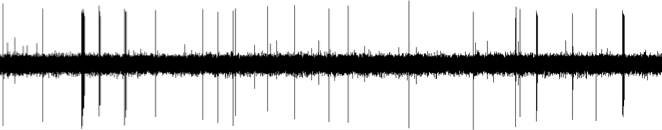
\includegraphics[width=0.49\columnwidth]{figures/Thalamus.png}}
    \subfigure[Zona incerta]{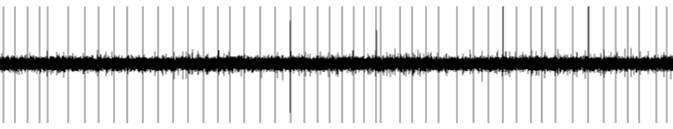
\includegraphics[width=0.49\columnwidth]{figures/Zona_incerta.png}}\\
    \subfigure[Nucleus subthalamicus]{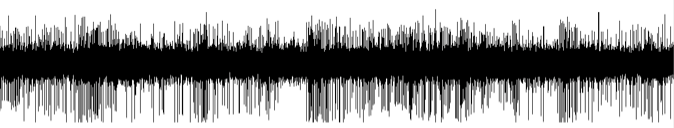
\includegraphics[width=0.49\columnwidth]{figures/nucleus_subthalamicus.png}}
    \subfigure[Substantia nigra]{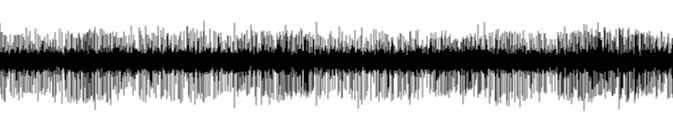
\includegraphics[width=0.49\columnwidth]{figures/substantia_nigra.png}}
    \caption{The MER discharge pattern changes depending on the functional region of the brain. The level of background activity and single-cell activity varies when entering or leaving specific regions and can be used to identify these region~\cite{Benazzouz2002,Hutchison1998}.}
    \label{fig:dischargepatterns}
\end{figure}

%MER is an intra-operative technique to gain information about functional areas of the brain. This information is gathered by inserting electrodes that measure the electric field properties created by the discharge of individual neurons in the surrounding tissue~\cite{McIntyre2006}. In the human brain there are a number of different types of neurons, which each have a distinct discharge behavior. The combination of those types leads to detectable discharge patterns that can be used to identify the region in which the measurement electrodes are located. Figure~\ref{fig:dischargepatterns} shows examples of the signals acquired from different brain regions. One possibility to distinguish the regions is to analyze the frequency of spikes within these signals. Usually this information is presented to the surgeon the raw  audio signal, an oscillogram, and as the result of a simple frequency analysis, e.\,g. a power density function. Based on this information the neurosurgeon can identify the current region and decide on how to proceed with the intervention. Different MER setups exist for measuring the electric fields. The system we used to record the data in this paper contains five electrodes with a square geometry in which the sides measure $1.5$mm and the fifth electrode is located in the center.

%As systems with different numbers of electrodes and geometries are available, our system is designed to handle different geometries and different numbers of electrodes. In order to prevent any confusion from the start, we chose to model the visual representations of the electrodes in such a way, that it is not consistent with any commercially available system. Otherwise, there might be the possibility that a surgeon recognizes our electrode representations of being type A, while they are in fact type B. Since he might deduct certain aspects from a specific electrode type, this mistake must be prevented.
%
%

\section{System Overview}\label{sec:overview}
%\begin{figure*}[t]
%    \centering
%    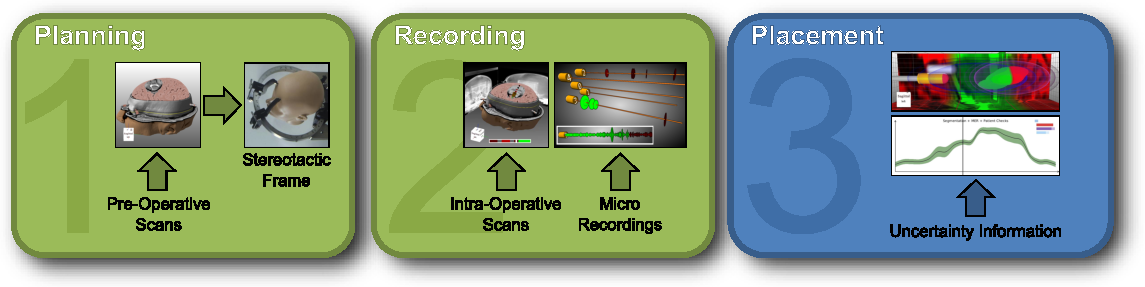
\includegraphics[width=0.9\linewidth]{figures/workflow}
%    \caption{The workflow of the proposed visual DBS intervention system can be divided into three phases: planning, recording and placement. To support each of these phases, we employ dedicated views which are arranged in a multiple view setup. External components interacting with our visualization system are shown for each phase.}
%    \label{fig:workflow}
%\end{figure*}

%Different MER setups exist for measuring the electric fields. The system we used to record the data in this paper contains five electrodes with a square geometry in which the sides measure $1.5$mm and the fifth electrode is located in the center.

The main goal of the designed system is to support the surgeon by reducing his cognitive load by fusing the available modalities and thus facilitating mental registration~\cite{Tory1998}. The current situation in the operating room is that the methods for inspecting the structural modalities, i.\,e.~MRI, CT, and biplanar x-ray scans, are fairly advanced and widely used. However, the systems for recording and analyzing the MER signals and patient checks are decoupled from the other modalities. By showing the temporal data of the recording in the spatial context of the scans, the surgeon is relieved of the burden of mental registration.

%Furthermore, the results of the patient checks, along with their uncertainty, are not accounted for in a formalized manner. By incorporating both modalities into a unified setup we support the surgeon in his decisions.

The second method, through which we support the electrode placement, is to present all collected data in a unified way and showing it in such a way that the optimal placement location is immediately visible and that the surgeon is guided towards it. The collected data consists of information about the intended target region, coming from the MRI scan, the MER recording, and patient checks.

%\subsection{Micro Electrode Recording}\label{sec:overview:mer}
%MER is an intra-operative technique to gain information about functional areas of the brain. This information is gathered by inserting electrodes that measure the electric field properties created by the discharge of individual neurons in the surrounding tissue~\cite{McIntyre2006}. In the human brain there are a number of different types of neurons, which each have a distinct discharge behavior. The combination of those types leads to detectable discharge patterns that can be used to identify the region in which the measurement electrodes are located. Figure~\ref{fig:dischargepatterns} shows examples of the signals acquired from different brain regions. One possibility to distinguish the regions is to analyze the frequency of spikes within these signals. Usually this information is presented to the surgeon the raw  audio signal, an oscillogram, and as the result of a simple frequency analysis, e.\,g. a power density function.

\subsection{DBS Intervention Procedure}\label{sec:overview:procedure}
Before proposing our system, we will first give a high-level overview of the DBS intervention procedure as it is specified in surgery guidelines~\cite{Hemm2010}. With respect to the steps in this procedure, a DBS intervention can be roughly divided into three subsequent phases: \emph{planning}, in which the intended target region is selected, \emph{recording}, in which the MER signal is obtained, and \emph{placement}, in which the emitting electrode is inserted, the patient checks are performed, and the placement is evaluated. %As these three phases define the overall workflow of a DBS intervention, they are used as the blueprint for the workflow underlying the presented system (see Figure~\ref{fig:workflow}).
%
%\begin{itemize}
%\item \textbf{Planning phase.} During this phase, the surgeon selects the intended target region and determines an optimal trajectory to access that region. We will describe how this phase is supported by the proposed system within Section~\ref{sec:overview:planning}.
%\item \textbf{Recording phase.} In this phase, the measurement electrodes are inserted into the brain, and moved towards the intended target region, while the electric field around them is recorded. This data is analyzed and the MER-based target region estimation is derived as described in Section~\ref{sec:overview:recording}.
%\item \textbf{Placement phase.} After determining the target position based on neuroanatomical features, and narrowing them further down using the MER measurements, the stimulating electrode is inserted into the target region, and the patient's cognitive and motor functions are tested, to get a more accurate estimate of the target region and find the optimal placement position. We describe the parts of our system dedicated to this process in Section~\ref{sec:overview:placement}.
%\end{itemize}
%
%To enable accurate navigation and data handling between the phases, more details about the DBS intervention procedure need to be considered.
%

As accuracy is of uttermost importance when performing DBS interventions, the patient is mounted into a stereotaxic frame that is rigidly fixed to the patient's skull. This frame has sockets that hold and precisely guide the equipment used during the intervention. Due to the known geometry of the stereotaxic frame, it serves as the basis for the coordinate transformation from imaging data to the patient. An important property of the frame is that it is visible in both, CT and MRI, scans and thereby serves as one of the landmarks used in the registration process. In the \emph{planning phase}, the surgeon plans the access path based on the pre-operatively acquired T$_1$- and T$_2$- weighted MRI scans. In most cases, however, the target region is not directly visible on either of the MRI scans and the surgeon has to rely on experience and patient-neutral heuristics to locate the target area. This step introduces some a priori unknown uncertainty into the position of the intended target region. %All these steps are performed within the planning phase of the DBS intervention. We will describe the visualization metaphors that we have developed to support this phase in Section~\ref{sec:overview:planning}.

%In the case of the STN, this is done as follows. First, the Talairach coordinate system is created based on the AC and PC regions and the mid-saggital plane, which are easily identifiable in MRI data~\cite{Talairach1993}. After defining this patient-specific coordinate system, a patient-neutral heuristic is used to find the STN target region relative to one anchor point, e.\,g.,~the PC. 

\begin{figure}[b]
    \centering
    \subfigure[Anterior-Posterior]{\fbox{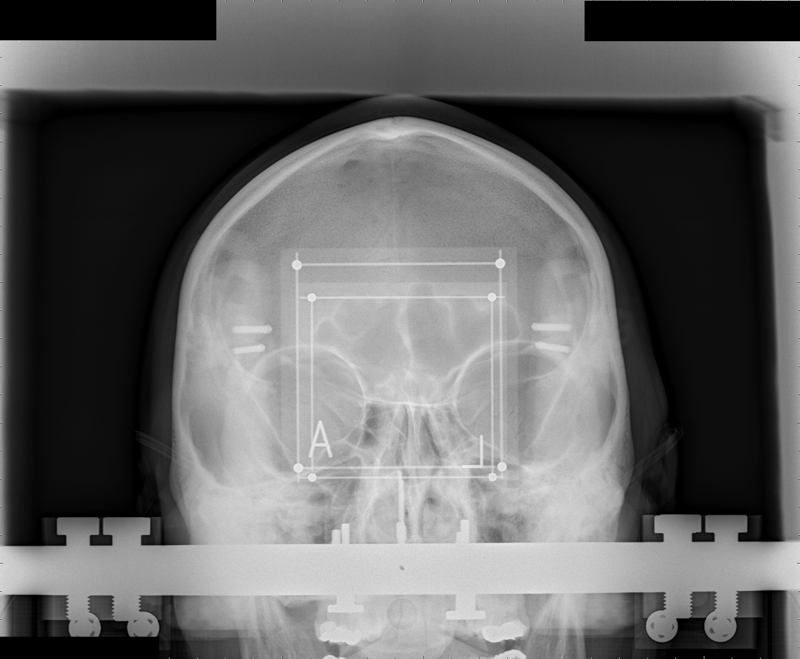
\includegraphics[height=0.4\linewidth]{figures/xrayslice-ap.png}}}
    \hspace*{0.1cm}
    \subfigure[Dorsal-Ventral]{\fbox{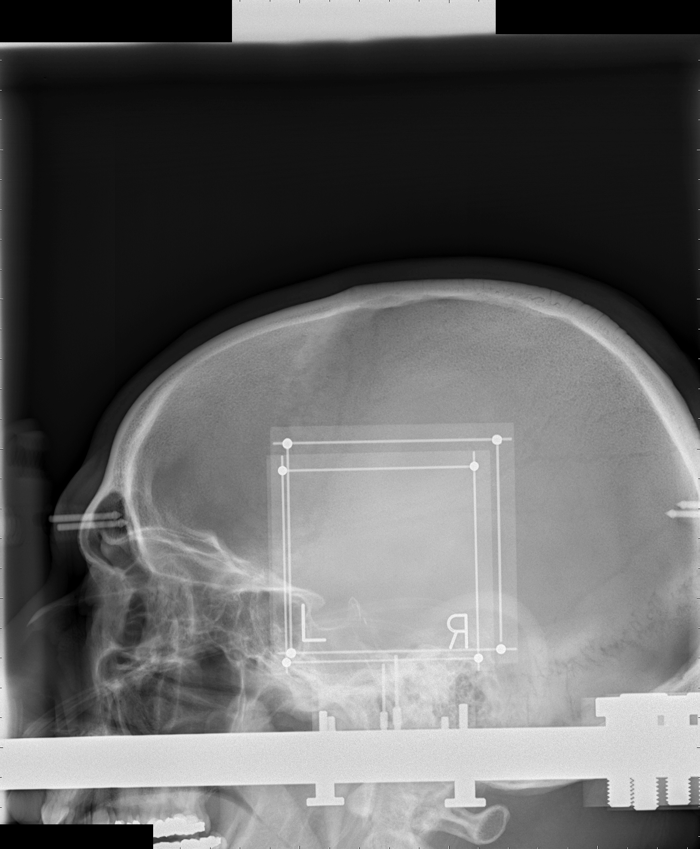
\includegraphics[height=0.4\linewidth]{figures/xrayslice-dv.png}}}
    \caption{Two x-ray images are created to calibrate the patient's position in the operating room using the perspective distortion of the reference plates. Subsequent x-ray images are used to verify the electrodes position inside the head and measure the uncertainty of the segmentation.}
    \label{fig:xrayreferencescans}
\end{figure}

Besides the pre-operative MRI scans, a pre-operative CT scan, and orthogonal reference x-ray scans  (see Figure~\ref{fig:xrayreferencescans}) are acquired. Following the scans the access path is drilled, the MER electrodes are inserted, and the recording is started. During the \emph{recording phase}, the electrodes are moved forward towards the intended target region while they continuously record the discharge pattern of the surrounding tissue. One member of the surgical team observes the signal, analyzes it, and informs the surgeon about the findings. We describe the developed visualization techniques supporting the recording phase in Section~\ref{sec:overview:recording}.

After the recording the MER electrodes are removed, the emitting electrode is inserted, and, in the \emph{placement phase},  the electrode placement is performed. Upon reaching the target depth the electrodes are activated and start emitting. Changing the position of the electrode, the surgeon tests the patient's higher brain functions in order to further narrow down the optimal electrode location. This is done based on expert knowledge on the positions of dedicated brain regions relative to each other. To monitor and verify this process and the electrode's actual position, orthogonal x-ray scans are obtained. We describe the visualization techniques developed to support the placement phase within Section~\ref{sec:overview:placement}.

%As these techniques show the data acquired before and during the intervention in a fused way, they can also be used to review the operation in a long-term, vertical, follow-up study. Over a long period of time, the cognitive and motor functions of the patients could be tested and rated. Ideally, the physician would want to perform a horizontal study as well, in which he can correlate the planned target location, the MER-corrected target location and the level of improvement to each other. This would enable iterative improvements of the heuristics, which surgeons use for DBS placements and lead to improved success rates.

\subsection{Planning Phase}\label{sec:overview:planning}
The goal of the planning phase is to identify the desired target region based on pre-operative scans, and to plan a trajectory reaching that target region by minimizing the distance to critical structures along the access path. There are a number of highly specialized tools available to perform this task, and there is also active research in the field of automatic trajectory planning~\cite{Shamir2010}. Since our focus is on other parts of the procedure, we implemented a basic planning tool, used to import the data from more sophisticated tools. The surgeon selects the intended target location and the burr hole position on a slice representation of the MRI scan. The resulting access path between the two selected points is shown in a 3D multimodal visualization of the pre-operative scans (see Figure~\ref{fig:recordingphase:3d}). As the 3D view contains all contextual information relevant during each phase of the DBS intervention procedure, it is used within all phases and serves as a red thread through the phases of the system.
%
%. First, the target region is selected on a slice representation of the MRI scan. Second, the entry point of the trajectory is selected, based on a 3D multimodal visualization of the pre-operative scans (see Figure~\ref{fig:recordingphase:3d}). As the 3D view contains all contextual information relevant during each phase of the DBS intervention procedure, it is used within all phases and serves as a red thread through the phases of the system.
%
%\subsubsection{Slice View}\label{sec:overview:planning:slice}
%\begin{figure}
%    \centering    
%    \subfigure[Slice View \label{fig:planningphase:slice}]{\fbox{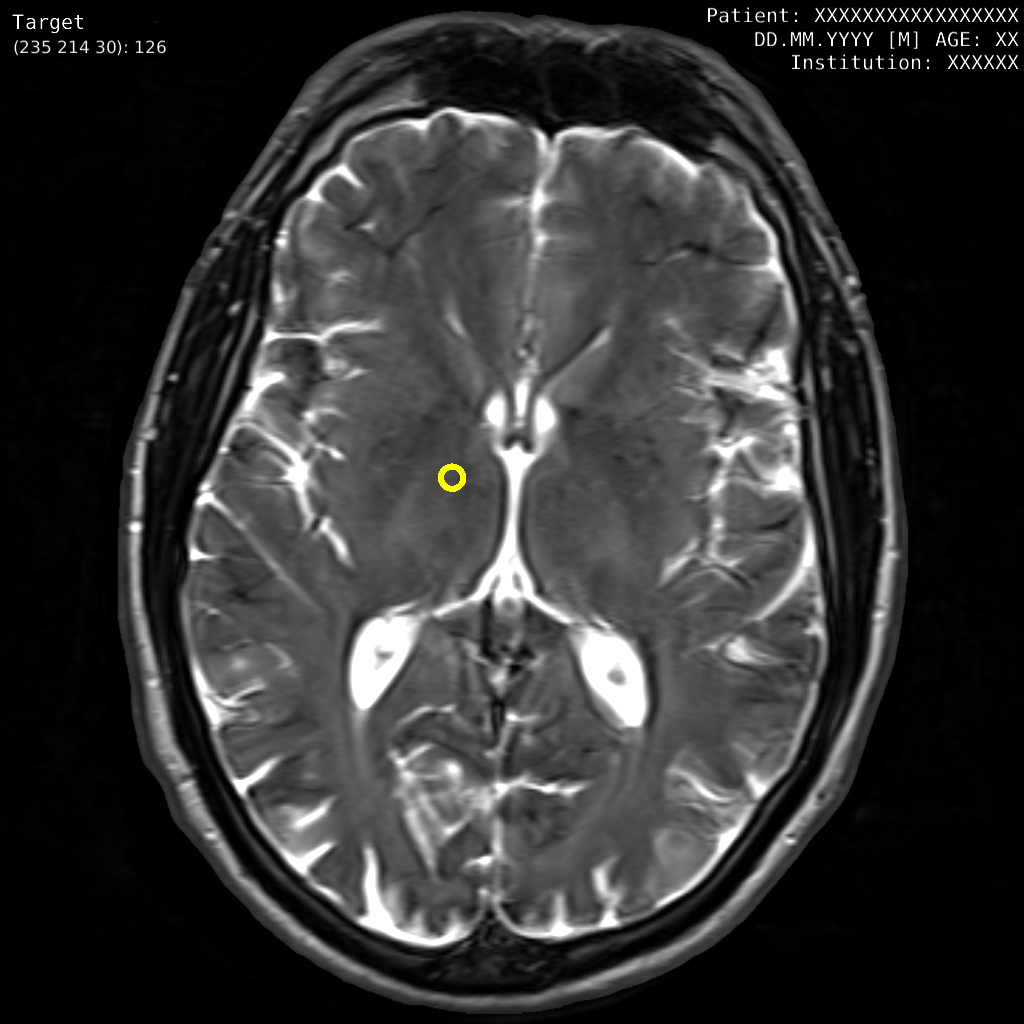
\includegraphics[width=0.45\columnwidth, height=0.45\columnwidth]{figures/planning-slice}}}
%    \subfigure[Contextual View \label{fig:planningphase:3d}]{\fbox{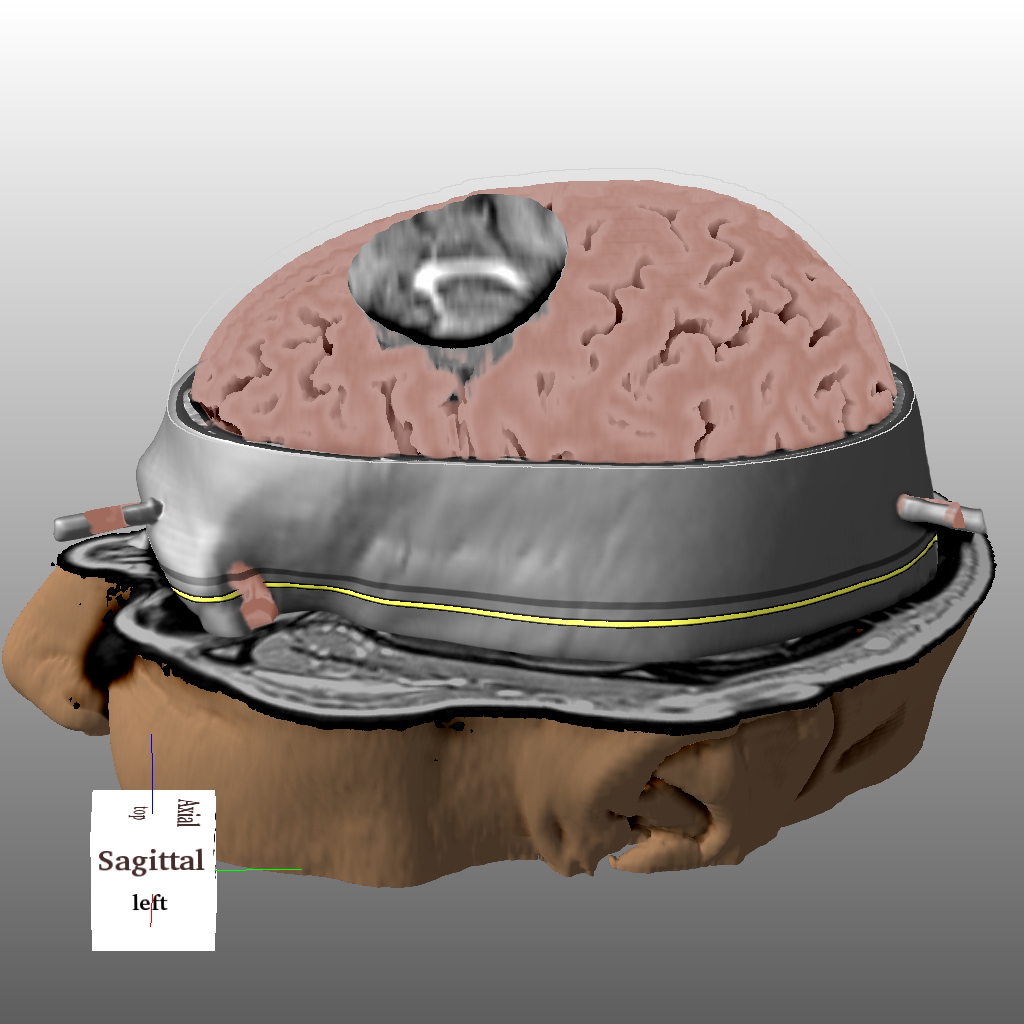
\includegraphics[width=0.45\columnwidth, height=0.45\columnwidth]{figures/planning-3d}}}
%    \caption{During the planning phase, two linked views are employed. A slice view helps to select the %target region (a), while a linked contextual view helps to interactively define the minimal invasive access path (b).}
%    \label{fig:planningphase:view}
%\end{figure}
%
%In the slice view (see Figure~\ref{fig:planningphase:slice}), the surgeon can browse through the slices of the two pre-operative MRI scans. Thus, this rather standard viewer allows for determining the probable location of the target region and identifying it at a sub-voxel accuracy. Even though, the pre-operative MRI scans are acquired at high resolution, the sub-voxel accuracy is crucial for accurate electrode placement, as the target region given by the STN spans only a few millimeters. Therefore, the neurosurgeon can pan and zoom within this slice view. Furthermore, the view presents the user with information about the intensity value at the selected point, and the patient's information in the upper right hand corner. The color of the marker in this view was chosen to provide a good contrast with the MRI signal, and allows mental registration with the slice indicator shown in the contextual view.

\subsubsection{Contextual View}\label{sec:overview:planning:3d}
The contextual view is the common element that is present in all three phases of our system. %This constant presence is useful as it creates a \emph{horizontal mental registration} between the different phases in addition to the \emph{vertical mental registration} present within each phase. %The latter is achieved by using this view as a frame of reference so that the individual information of the other views can be related to the common contextual view.
It is based on a multimodal visualization of the pre-operatively acquired CT and MRI scans. To improve spatial comprehension, the three modalities are not fused but vertically separated such that, for each layer, the modality of highest interest is visible (see Figure~\ref{fig:recordingphase:3d}). At the lowest layer we render the T$_1$-weighted MRI with a transfer function that shows the whole head of the patient. The spin-lattice time was chosen since it allows for an easier classification of the skin and the relatively stable gradients allow for reasonable shading. This part communicates the orientation of the patient intuitively and thereby reduces dangerous left-right mismatches by the surgical staff. The cut-off line between this layer and the next can be interactively moved by the user to enable data inspection. The lower layer is capped with a slice view that provides the surgeon with direct access to structural information embedded within the spatial context. The skull is partly visualized in the middle layer, based on the CT scan, to serve as a smooth transition between the lower layer and the brain. To obtain an occlusion-free view to the brain we employ a skull stripping approach, described in Section~\ref{sec:implementation}, at the highest layer. As MRI has a low signal-to-noise ratio, gradient-based shading is not viable when visualizing the brain. Instead, we employ depth darkening~\cite{Luft2005}, which increases the depth perception of the brain's structures. The depth of the intended target region is visible as a yellow band surrounding the skull and serves as another depth cue.

We present the access path to the surgeon by removing the structures around the trajectory~\cite{Weiskopf2002,Rieder2008}. The removed area is cylinder-shaped and possesses a variable, user-defined radius so that the surgeon can inspect the walls of cylinders with varying radii. To increase the amount of information the surgeon gains from the cylinder walls, the same transfer function as used in the slice representations is applied here. This increased access path radius gives the surgeon access to more information in a spatial context.
%So far, all the described features of the contextual view are common to all three phases. However, the specialty in this phase for the contextual view is, that it also indicates the slice which is currently viewed in the slice view, as a dark gray band projected onto the head. Based on this band, the surgeon can immediately see at which depth the currently viewed slice is located. While any surgeon will possess the knowledge to roughly infer this information from the surrounding tissue or by comparing the number of total slices to the current slice number, both methods require conscious or subconscious mental processing which should be avoided. Perceiving a band projected to the 3D structures is a much more intuitive way requiring potentially less cognitive effort, such that the surgeon can focus on locating the target region.

\subsection{Recording Phase}\label{sec:overview:recording}
The recording phase is the next step during a DBS intervention following the opening of the patient's skull. While moving the electrodes deeper towards the target region, each detects the signals from the surrounding tissue and transmits them to the controlling device. To obtain knowledge about the current region, the received signals are constantly analyzed and classified.

%\subsubsection{MER Signal Analysis}\label{sec:overview:recording:signalanalysis}
%The MER signals are highly corrupted by noise, as the transmission is followed by an amplification of around three orders of magnitude, i.\,e.,~from $\mu V$ to $V$, which introduces $1/f$ wideband random component noise. In our system, also another type of noise was detected, a set of sinusoidal or very narrow band signals pitched at constant frequencies. While the $1/f$ noise is justified by thermal noise in the amplification system, which reaches critical levels, the origin of the sinusoidal components is unknown and probably due to interference with other equipment used during surgery. The $1/f$ noise has amplitudes comparable to the neuron pulses to be detected, while the latter are still audible in the auditory analyses.
%
% KEEP  ?? REMOVE ??
%In order to better condition the signal for audio analysis and thus for visualization, we tapered the amplitudes of the sinusoidal noise components. This was achieved by means of a set of notch filters tuned at the frequencies of the sinusoids. In order to reduce the impact of the denoising process, we decided to eliminate only the most prominent sinusoidal components. Sinusoidal tapering was achieved as follows. First, the frequencies of the sinusoids were detected by means of a peak picking algorithm, then a set of band stop Type I Chebyshev filters were designed, one for each frequency. In order to guarantee the stability of the design and effectively eliminate the sinusoidal components, we found it optimal to use filters of order six, with a stop band margin of $1\%$ of the sampling rate and stopband centered at the detected frequencies of the sinusoids, and ripple of $0.1$ dB. The neuron firing signal being wideband guarantees that the introduction of small band gaps has no other acoustical impact than reducing discomfort and distraction due to the presence of the sinusoids. Since the $1/f$ noise and the neural firing signals are both wideband and have comparable amplitude, we did not attempt direct removal of this noise component, in the effort of minimizing the deterioration of the signal. Other methods have been proposed for the same means~\cite{Jansen,Donoho1995}, but we found our method to be sufficient for the handled recording data.

%In the target region, the amplitude of the neuron firing signal is higher than that of the noise floor. For automatic detection and visualization purposes a threshold on the noise floor is estimated in zones where the neuron firing signal is not present. Applying this threshold to the instantaneous signal amplitude in the time domain has then the effect of revealing and enhancing the peaks of the neuron firing signal when they are present. Based on this signal, 

Possibilities exist to automatically detect the region. The analysis and computation of these metrics, however, is not in the main focus of this paper, so this it is not elaborated on in detail. Instead, any of the following variants can be chosen and a comparative study might be the focus of future work. One possible set of metrics consist of the firing rate, burst index, pause ratio, and the pause index, which were introduced by Haese et al.~\cite{Haese2005}. They also determined, that these metrics are useful to map the signals to specific brain regions. These values are computed using the denoised signal and applying a non-linear energy operator as presented by Maragos et al.~\cite{Maragos1993} and a spike detection with a subsequent thresholding presented by Mukhopadhyay et al.~\cite{Mukhopadhyay1998}. As several other comparable approaches exist, for our setup it makes no systematical difference, which of the classification algorithms are used.

\subsubsection{Additions to the Contextual View}\label{sec:overview:recording:3d}
\begin{figure}
    \centering
    \fbox{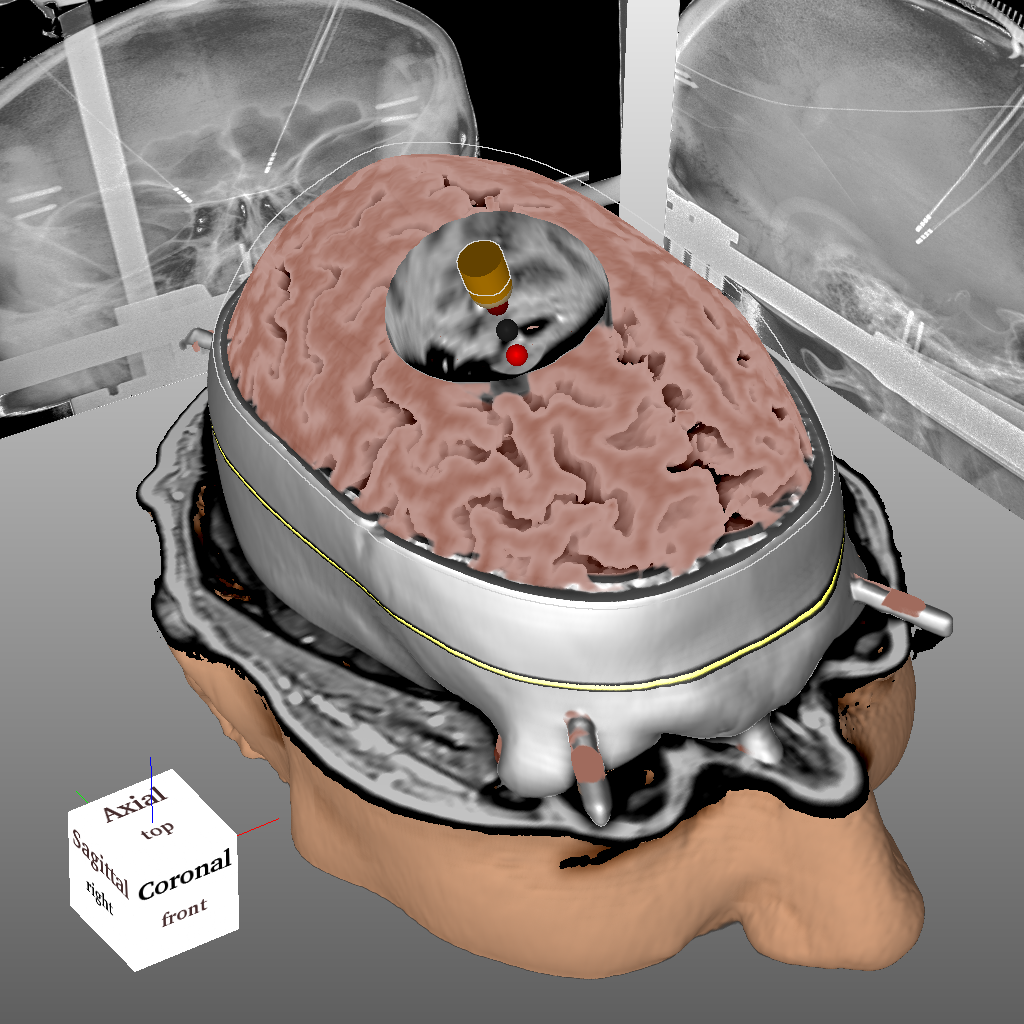
\includegraphics[width=0.9\columnwidth]{figures/recording_3d}}
    \caption{In the recording phase the contextual view additionally shows the intra-operatively acquired x-ray scans. It further shows the electrode while it is begin advanced towards the target. The beads behind the electrodes show the results of the MER signal analysis.}
    \label{fig:recordingphase:3d}
\end{figure}

The contextual view as employed in the recording phase is, in most parts, identical to the one used in the planning phase. However, as this phase of the intervention process requires additional information the view differs in some ways. First, since the current depth of the MER electrodes is known, we can compute and display a representation of the electrodes. As the extent of the electrodes is very small compared to the whole head, and we are only interested in the general position and orientation of the electrodes, just a single representative proxy electrode is rendered. 

Using the MER signal analysis, we can classify depth values by their functional areas. Doing this continuously for every point along the access path would introduce a lot of visual clutter that would not give additional insight but rather confuse the user. Therefore, we classify and summarize segments along the trajectory that we can classify up to an acceptable certainty. For each classified segment we display a visual representation, to which we refer as a \emph{bead}, in the center of the canal at that specific position. Each bead is rendered as a shaded sphere with a specific color. This visual metaphor has been proposed before~\cite{Miocinovic2007,Haese2005} and provides both contextual and functional information. The bead's color correlates to the classified region. A black bead is created if there has been a longer distance without a reliable classification. These intermediate beads are important to maintain the analogy of a bead string, helping the user understand the spatial relationship. Different shades of red are used for areas that lie outside of the desired target area. It is important to present this information to the surgeon as he can deduce more information from the changes between different areas. The first choice for a color would be different shades of gray, since it does not draw as much attention. But since the canal wall is gray and the human visual system is not adapted to differentiate gray tones, we chose red as the hue for these regions. As soon as the analysis of the spike signals indicates that the MER electrodes are in the target region, green beads are rendered that draw attention to those structures. Furthermore this color coding resembles the traffic light color scheme proposed by Rieder et al.~\cite{Rieder2010}, which intuitively assigns green to {\it good} areas, while red is assigned to {\it bad} areas. To further reduce visual clutter only one bead is rendered for all electrodes. This is a viable simplification as the different functional regions of the brain are oriented such that either all electrodes detect the same signal (either type of tissue or undefined) or a subset of electrodes detects a regional signal and the others detect an undefined signal.

Even with the application of the depth darkening shading technique described by Luft et al.~\cite{Luft2005}, the depth perception of the electrode is not optimal. One possible solution would be the introduction of a distance ring as described by Rieder et al.~\cite{Rieder2008}. Instead, to reduce occlusion within the focus of the view, we decided to show a linear scale outside of the view's focus where it does not block any relevant structures. The vertical white bar in this scale gives immediate feedback about the electrode's position. This widget is the first visualization used within our system, which employs a \emph{normalized view}. It means that the left-most position in the view corresponds to the entry point of the access path and the right-most position is slightly further than the intended target region. As soon as a functional area has been detected the background is colored with the respective color as well. Even though the beads convey a good absolute spatial orientation their relative orientation is not immediately obvious for occlusion and perspective distortion. On the other hand, the distance widget does not contain any information about the absolute location. The combination of the beads in the contextual view and the color in the distance widget provide the relevant information to the surgeon.

Another addition to this view is the inclusion of the intra-operative x-ray images, which can be easily registered to the patient using the external and internal camera matrices and the known geometry of the two reference plates, which are shown in Figure~\ref{fig:xrayreferencescans}~\cite{Caprile1990,Zheng2008}. Using the complete camera matrix, it is possible to select a point in both images and reconstruct, up to a certain accuracy, a 3D position within the volume from it~\cite{Hartley2004}. On demand the position of the reconstructed electrode position will be shown in this view by rendering a second electrode in gray that is blurred to accommodate for the uncertainty. The specific uncertainty is, among other things, dependent on the geometry and resolution of the x-ray detectors and is therefore different for each operating room. In our test case the position is in the order of $< 1$mm. As these x-ray scans are used to guide the surgeon on his way to the target region and provide one important possibility to verify the final position of the electrode, the integration with the other spatial modalities is important. In addition, we use the discrepancy between the expected electrode position and the reconstructed position as an uncertainty for the target region's segmentation in the later phase.

%
%\subsubsection{Multi-Planar Slice View}\label{sec:overview:recording:mpr}
%
%\begin{figure}[t]
%    \centering
%    \fbox{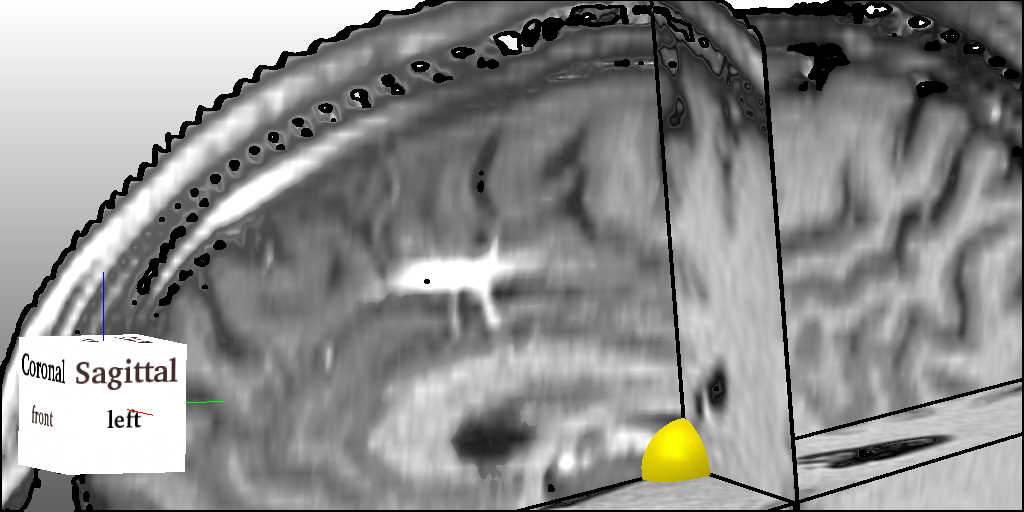
\includegraphics[width=\columnwidth, height=0.5\columnwidth]{figures/recording-mpr}}
%    \caption{The Multi-Planar Slice View shows the position of the MER electrodes in the context of the surrounding tissue. The orthogonal slices are oriented so that one plane caps off the canal and another lies in the midsaggital plane, while the third plane is perpendicular to both others. The intended target region resides in the intersection of the three planes and is represented by a small sphere. The current position of the electrodes is shown by a disc in the same color as the electrodes.}
%    \label{fig:recordingphase:mpr}
%\end{figure}
%
%The multi-planar slice view shows three orthogonal slices centered on the intended target region. Its main purpose is to allow a better occlusion-free depiction of the current's electrode position and orientation in relation to the planned target region. The beads are visible in this view as well, but in addition to the other views in which they are present, each electrode's signal is analyzed on it's own. This way, the surgeon can inspect the different analyses of the signals in more detail and can gain deeper insight. To depict the electrode placement, a disc is shown at the current electrode's tip position. As this disc communicates the current position, the size of the tip and the beads are not crucial in this view, and can thus be enlarged for better identification. While this enlargement results in an increased occlusion, this poses no problem, as identification of structures around the electrode is performed in the detail view discussed further below.
%
%The slices of the multi-planar slice view lie in the coordinate system defined by the the canal axis, the midsaggital plane, and the cross product of those. To reduce the degree of occlusion introduced by the opaque slices, two of the slices are clipped, such that irrelevant regions are discarded. This, among others, focuses the user's attention on the central structure of the image, which contains the intended target region. The third sagittal slice is not clipped, in order to preserve the structure context as well as coherency with the contextual view.


\subsubsection{2D Temporal Audio Visualization}\label{sec:overview:recording:mer}
\begin{figure}[b]
    \centering
    \fbox{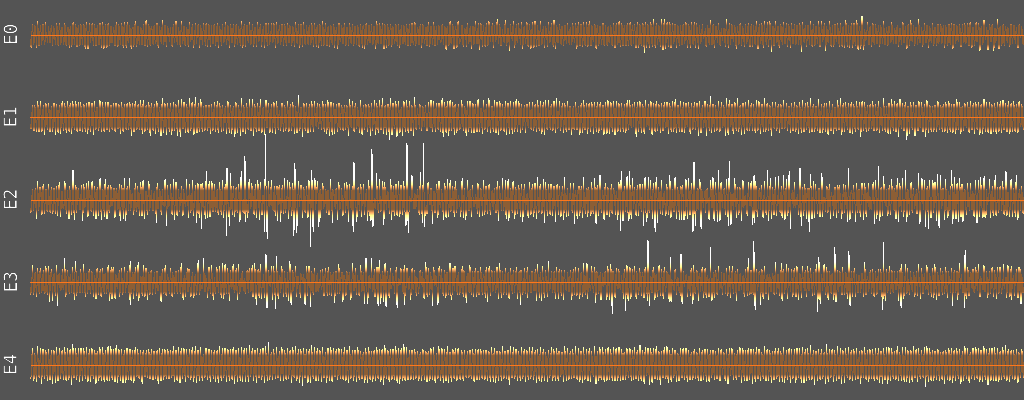
\includegraphics[width=\columnwidth, height=0.5\columnwidth]{figures/audio_signal.png}}
    \caption{The MER signal in the time domain is shown using an oscillogram-like representation in which time is on the horizontal axis and the electric potential difference on the vertical. The visual perception of the signal is enhanced by de-emphasizing the background noise and guiding the attention to the more important spikes. The signal of the currently selected electrodes is highlighted.}
    \label{fig:recordingphase:sound}
\end{figure}

In this view we present the raw data collected by the MER electrodes in real time. One graph is shown for each electrode, which shows the electric potential difference plotted over time. The scaling factor of the ordinate can be manually adjusted to account for patient and equipment specific differences. The identifying names for each electrode are shown on the left hand side next to the graphs.

Since surgeons are generally more interested in the distribution of spikes than the background noise, we visually enhance spikes such that they are the immediate focus of attention. This visual enhancement is done by defining a threshold value below which all values are de-emphasized, i.\,e.,~a darker color is chosen and above which the values are emphasized with a brighter color. There is an exponential transition in the area around the threshold to reduce any unwanted attention that would otherwise result from a discontinuity. This threshold value can be varied by the user to include a wider or narrower range of values in the focus area. The color scheme matches the color on the electrode representations and at the same time intensifies the perceptual distance between the colors used for the thresholded area and the spikes.

To facilitate linking between all views containing a representation of the MER signal further, the surgeon can select electrodes which are then highlighted in all views (see Figure~\ref{fig:recordingphase:sound}). A problem with current systems is that the surgeon must maintain a mental model relating the horizontal oscilloscope graphs with the geometric orientation of the electrodes within the patient's head. By creating a linked view between those two representations, we reduce the mental burden on the surgeon without preventing him access to any of the information.

\subsubsection{3D Spatiotemporal Audio Visualization}\label{sec:overview:recording:3daudio}
\begin{figure}[t]
    \centering
    \fbox{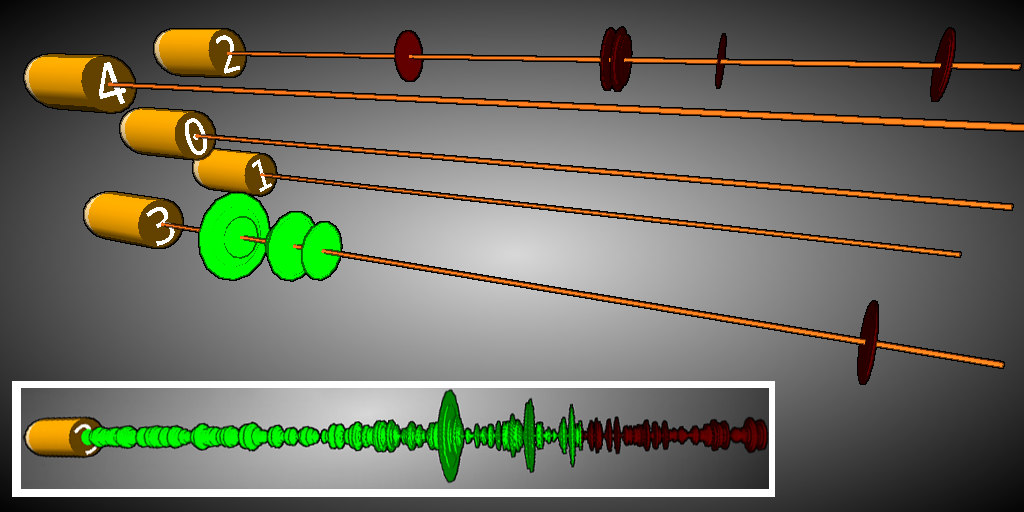
\includegraphics[width=\columnwidth, height=0.5\columnwidth]{figures/recording-3dsound}}
    \caption{Fusing the spatial orientation and layout of the recording electrodes with the temporal signal relieves the surgeon of the burden to keep this association in mind. To enhance the perception of the spikes, only the values above a certain threshold are shown in this view so that they are visible pre-attentively. The picture shows the same signal for subsequent time steps. The inset shows the result for one electrode without thresholding.}
    \label{fig:recordingphase:3dsound}
\end{figure}

%The electrodes follow the camera movement of the contextual view but remain oriented in the way they actually are within the patient. This way, the surgeon does not need to keep the orientation of the electrodes in mind and can more easily the structural information with the MER time domain.
It is important to bridge the gap between the MER signal, defined over the time domain, and the structual data, contained in the imaging data. We achieve this by employing an audio visualization that directly combines the spatial information of the electrodes with their temporal electric signal. Each electrode shows its electric signal as concentric discs around the centerline. The discs start at the back end of the electrode with a radius that scales linearly with the absolute value of the amplitude. As soon as the next measurement is registered the discs move away from the electrode and a new disc is inserted at the back end. This way the signal originates from the electrode and moves away from it over time. Considering the absolute value of the amplitude is sufficient as the spikes are distributed symmetrically and surgeons are not interested if the spikes occur because of a negative potential difference or a positive one. The discs are distorted since they are drawn perspectively. This is not a serious problem because, on the one hand, the actual amplitude of the signal is not as important as the frequency of the signal and, on the other hand, the 2D signal is presented to the surgeon as a backup as well.

Creating a disc for every measurement point would clutter the whole view (see inset in Figure~\ref{fig:recordingphase:3dsound}). Therefore we apply the same thresholding technique as described in the previous section, but discard all signals which lie below the threshold completely.

%In the 2D case the color was used to separate the thresholded values but since we only keep the spike values, we can use the results of the analysis from Section~\ref{sec:overview:recording:signalanalysis} to color and shade the visualized discs.

\subsection{Placement Phase}\label{sec:overview:placement}
In the placement phase the surgeon needs to consider all acquired information to decide on the optimal position of the stimulating electrode. This decision is based on three different factors that are all affected by varying uncertainties.

First, his experience and knowledge by selecting and segmenting the intended target region during the planning phase. The segmentation is uncertain as, for example, the brain shifts from its scanned position during the operation. There exist techniques to reduce this uncertainty and we estimate this uncertainty by measuring the difference between the expected electrode position and the reconstructed position based on the x-ray images. Second, the results of the MER recording and the area along the trajectory. The uncertainty for this step is highly dependent on both the algorithm used to analyze the MER signal and the electrode configuration. The third factor is acquired when the stimulating electrode is inserted and activated. The surgical staff will test different brain functions of the patient. Since it is well-known which areas affect which capabilities while stimulated, the surgeon can further narrow down the location of the optimal target region. In our example we use two brain functions, the ability to recall events from long-term memory and an increase in tremor of the patient's hand. Each of the functions is tested separately along the access path and, based on the surgeons experience and a user-neutral heuristic, it is possible to deduce the position of the target region relative to the measurement point. The level of uncertainty for this information is relatively constant and in the same range as the extent of the electrodes, i.\,e.~$< 1.5 mm$ for our setup. For each decision factor we independently measure the probability, and uncertainty, of the target region's position along the access path.
   %To aid in this final phase, we provide the surgeon with five different linked views. In contrast to the recording phase, where there were five recording electrodes, the surgeon only inserts a single stimulating electrode in the placement step, so that only a single electrode is presented in each view.

The contextual view introduced above is shown to maintain the surgeon's mental registration. However, since the whole trajectory has been measured in the previous phase all beads and all information previously acquired in the canal tube is presented independent of the electrode position. 

%\subsubsection{Spatial Audio Visualization}\label{sec:overview:placement:spatialaudio}
%\begin{figure}[t]
%    \centering
%    \fbox{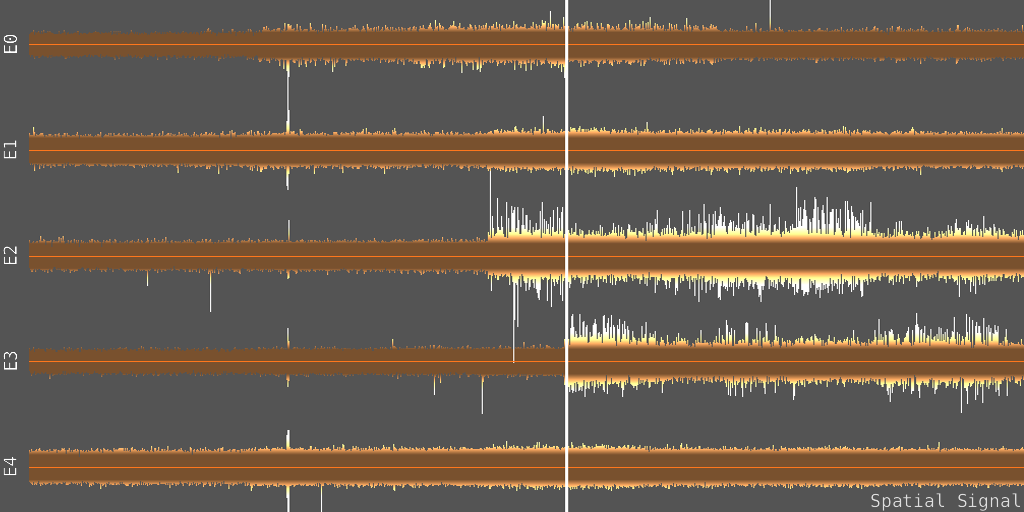
\includegraphics[width=\linewidth, height=0.5\columnwidth]{figures/verification-sound.png}}
%    \caption{For the placement phase, it is necessary to inspect the MER signal based on the location where it was recorded, rather than depending on the time. This view is a normalized view, which shows the entry point on the left and the desired target region on the right. The visual enhancement is not as extensive as in Figure~\ref{fig:recordingphase:sound} since the preattentive perception is not as important here.}
%    \label{fig:placementphase:spatialsound}
%\end{figure}
%
%This view similar to the temporal audio visualization discussed above. The important difference, however, is that this graph does not plot time against amplitude, but rather position, i.\,e.,~depth, vs. amplitude. The view is a \emph{normalized view} as defined above. Similarly as in the temporal audio visualization, a modifiable threshold can be applied, which has a special importance in this view since the surgeon inspects all values at the same time and might miss important data because of the visual clutter, which would be otherwise occur.
%
%\subsubsection{Canal View}\label{sec:overview:placement:canal}
%
%\begin{figure}[b]
%    \centering
%    \fbox{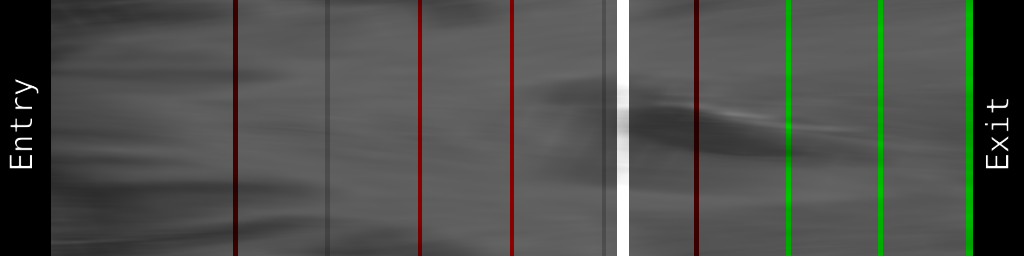
\includegraphics[width=\linewidth, height=0.25\columnwidth]{figures/verification-canal.png}}
%    \caption{The canal view presents the surgeon with a representation of the tissue within a cylinder centered on the trajectory. This allows for occlusion-free inspection of the MRI signal in all directions simultaneously. The current depth of the electrode and the analysis of the MER signal are shown as an overlay to provide easy registration.}
%    \label{fig:placementphase:canal}
%\end{figure}

%The canal view provides access to information about the tissue surrounding the planned trajectory (see Figure~\ref{fig:placementphase:canal}). It is a normalized view with the entry point on the left side and the target region on the right, such that mental registration is easily possible with the spatial audio view. The canal view is generated by casting rays from a cylinder surface centered on the trajectory to another centered cylinder surface. The canal view is generated through regular volume raycasting, whereas the entry and exit points have been modified to fit the cylindrical geometry. Thus, the image of dimensions $X$ and $Y$ is a 2D presentation of the cylinder points in polar coordinates. That means that the axis of the cylinder is subdivided into $X$ concentric rings, with each point representing an angle of $2 \pi / Y$. This way of presenting the area surrounding the trajectory allows the surgeon to analyze the data occlusion-free, and into all directions simultaneously. In order to create the vertical mental registration, the current depth of the electrode as well as the detected regions are shown as overlays. The regional overlays are just thin stripes instead of areas, so that they do not occlude any detail which is shown below. To further explore the structures surrounding the access path, the diameter of the two cylinders used to generate the canal view can be varied. 

\subsubsection{Target Closeup}\label{sec:overview:placement:targetareaview}
\begin{figure}[t]
  \centering
  \fbox{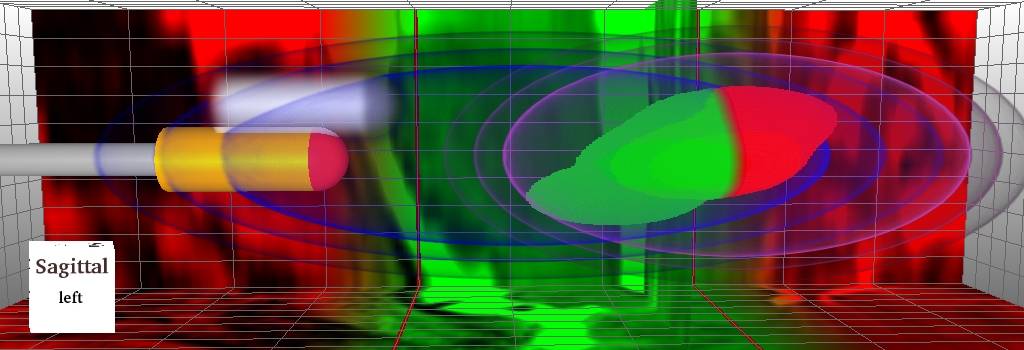
\includegraphics[width=0.98\columnwidth]{figures/electrode_closeup.jpg}}
  \fbox{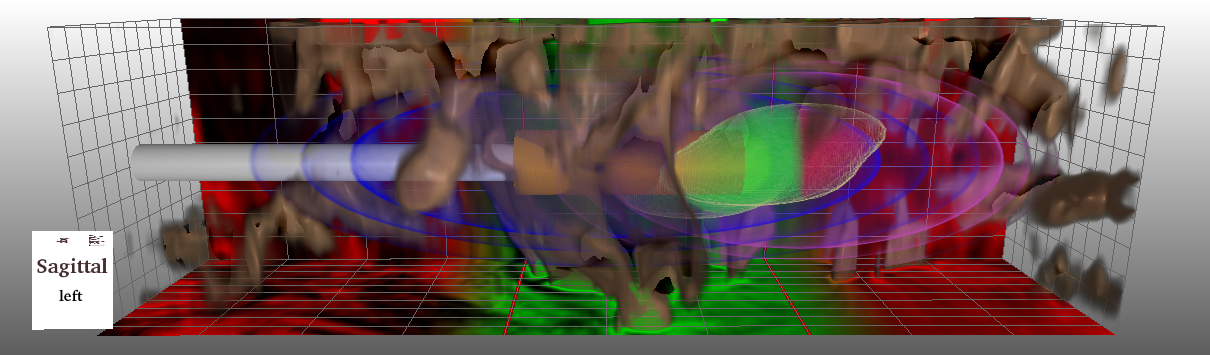
\includegraphics[width=0.98\columnwidth]{figures/target-region_full}}
  \caption{The target closeup visualization shows the potential target regions (planned=yellow, speech tests=blue, movement tests=purple). The spatial context provided by the MRI signal is color coded using the red-green MER region mapping. The stimulation electrode changes its color when it is entering the intersection of the potential target area.}
  \label{fig:targetregion}
\end{figure}

The localization procedure must not only communicate the electrode's position with respect to anatomical structures, but also with regard to the intended target region. An optimal placement of the stimulation electrode should be in the intersection of the potential target regions obtained from the different measurements. We support this in-detail navigation aspect by providing a 3D visualization, to which we refer as \emph{target closeup}, that shows the electrode embedded within the potential target regions together with the intended target region. To relate these potential target regions to the electrode and embed them into the spatial context, we additionally display the pre-operative MRI scans as a view-dependent projection on the back faces of the target closeup's bounding box. The rendering of the datasets has been made optional, as it on the one hand can provide valuable information regarding the intersection between the electrode and structures of interest, but on the other hand also occludes the potential target regions. The same orientation overlay is used in the electrode closeup, which is also used in the other 3D representations, to allow a seamless embedding of this view.
%To support the placement process multiple potential target regions and their intersection are shown in a fused manner. These potential target regions are: the pre-operatively planned one using the MRI data, the one derived from the MER measurements, the information from the x-ray scans, and the regions derived from the patient tests, e.\,g. speech, memory and movement.

We have to deal with three different types of potential target regions, whereby the type of a region is dependent on the way it has been acquired. First, the \emph{planned region}, which has been manually defined through segmentation by the surgeon on the basis of the pre-operative MRI scan. Therefore, we can apply volume rendering to show the result of this planning process. The second type of potential target region is derived from the \emph{MER signal} and has considerable uncertainty. This is projected onto the bottom plane of the detail view with the color coding which we have also used for visualizing the original MER signal. A user-defined safety margin is displayed to account for the occurring uncertainty sources. The third type of potential target region derive from the \emph{patient tests} performed when placing the actual stimulation electrode. As the patient checks are conducted during the electrode placement phase, the corresponding regions are changeable interactively. The region is shown as an ellipsoid in 3D assembled by connecting several check points. In the example shown in Figure~\ref{fig:targetregion}, we depict the ellipsoid generated from multiple speech tests in yellow, while the ellipsoid obtained from the movement tests is depicted in blue. The safety margins are depicted by using transparency, as it allows to communicate them intuitively while still maintaining a moderate level of occlusion. The width of the safety margins can be changed interactively by the surgeon and is dependent on experience and the electrode configuration that is used in the intervention.

Similar to the contextual view, we give the surgeon the possibility to show the approximate location of the electrode as reconstructed from the x-ray scans. It is of special interest in this view, as shows it the deviation from the predicted electrode position, due to brain shift and minute bending of the needle, from its actual position. The uncertainty is shown by blurring the rendering of the electrode to fill the size of the uncertain region.

Finally, we have to emphasize the intersection of the displayed target regions, as this intersection is the region where an optimal electrode placement would occur. We compute this intersection interactively and visualize it volumetrically with a green hue, the same which is also used for the green-to-red MER mapping. This way, the surgeon can verify the overlap and decide individually which region to place the electrode in. Furthermore, through the extent of the red region, the surgeon gets information about the mismatch between the pre-operative planning and the MER recordings. To further guide the surgeon during the electrode placement, we additionally change the color of the electrode when it penetrates the computed interaction of the potential target regions.

\subsubsection{Placement Guide}\label{sec:overview:placement:guide}
\begin{figure}[t]
  \centering
  \fbox{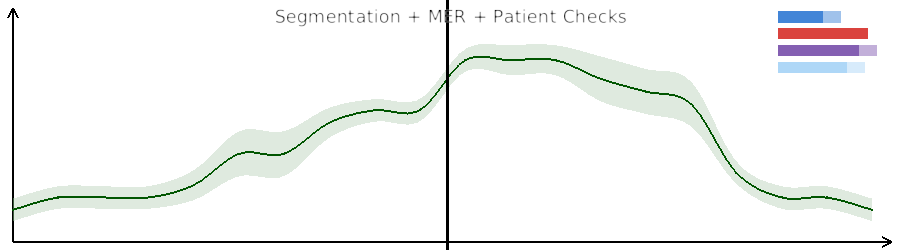
\includegraphics[width=0.96\columnwidth]{figures/segmentation_mer_patientchecks.png}}
  \fbox{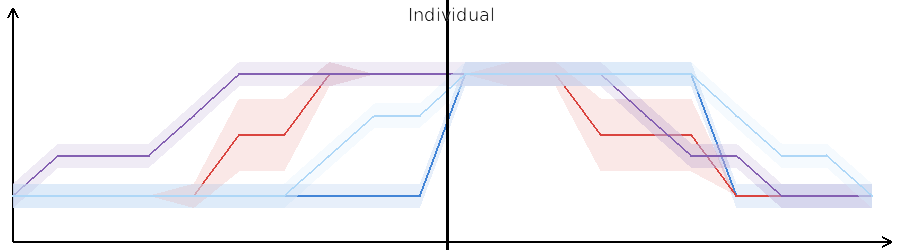
\includegraphics[width=0.465\columnwidth]{figures/individual.png}}
  \fbox{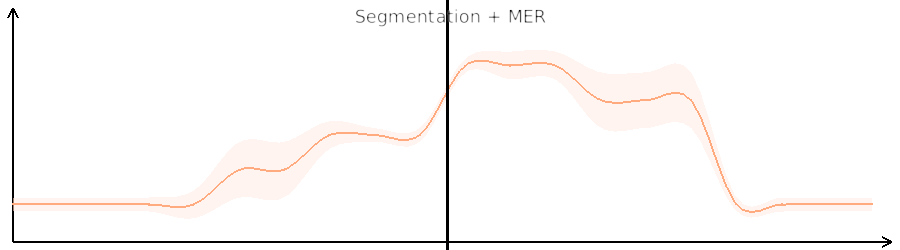
\includegraphics[width=0.465\columnwidth]{figures/segmentation_mer.png}}\\
  \fbox{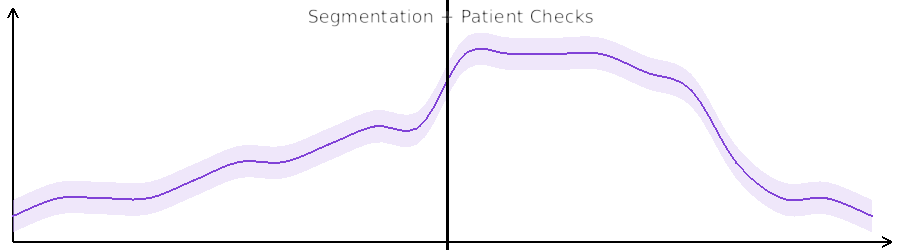
\includegraphics[width=0.465\columnwidth]{figures/segmentation_patientchecks.png}}
  \fbox{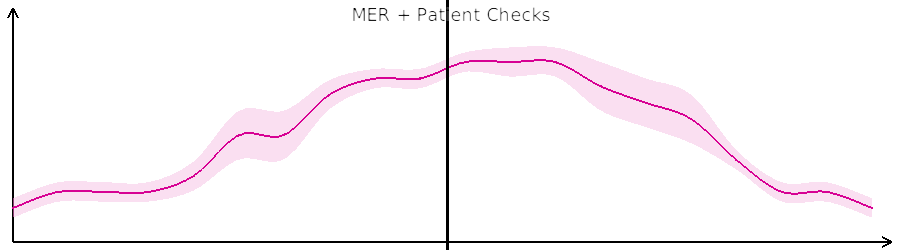
\includegraphics[width=0.465\columnwidth]{figures/mer_patientchecks.png}}
  \caption{The placement guide gives a quantitative overview of measured data for potential target regions. The top figure is a combination of all data values, where as the lower figures present detailed information by showing either all values or pairwise combinations. These combinations allow the surgeon to gain further insight into the measurements in certain situations, for example, when a measurement proves unreliable during the procedure.}
  \label{fig:placementguide}
\end{figure}

In addition to the spatial context, as described in the previous section, we also present the potential target regions quantitatively in a view we call \emph{Placement Guide}. This view is centered on the intended target region with the access path depth on the abscissa and the likelihood of the actual target region on the ordinate. By showing the quantitative data in a line plot, the surgeon immediately sees in which areas most of of the measurements agree and is visually guided towards that position. As we have multiple decision values for each depth value, we can combine them in different ways. In our example we chose a weighted sum in which every weight can be selected by the surgeon. The combination function can be, however, freely exchanged according to future research. The values for uncertainty are combined in the same way and are rendered as transparent areas surrounding the line. Transparency has been shown to be a good way to convey uncertainty in other contexts~\cite{Djurcilov2002239}. With this representation the size of the transparent area immediately shows how uncertain a specific value is. This allows the surgeon to see the whole set of information at one time and decide on an optimal placement position. All combined views use spline-based smoothing on the curves, which can be disabled by the user on demand. This is done so that the surgeon is not distracted by abrupt changes in the data values that would otherwise draw unwanted attention . The current position of the electrode is shown as a vertical bar in each of the views.

The top figure in Figure~\ref{fig:placementguide} shows the combined data of all values and is of central interest for the surgeon. It provides an overview of all measured data and guides him to the most likely, i.\,e.~highest, position. The curve will be assembled interactively while the stimulating electrode is being advanced and the patient checks are performed. Since the combined curve hides possible outliers and gives no feedback on the underlying values, the composition of each sample point can be examined in the top right as a bar plot that shows the probability and uncertainty for each decision factor separately. All bars are justified to the left and their width directly relates to the measured value. As with the line plot, a transparent box shows the area of uncertain values. One bar is rendered for each source of measurements, so that in our case (see Figure~\ref{fig:placementguide} there is one bar for the segmentation, MER, and one for each of the two patient checks. Including a line alongside the combined data for each of the decision factors would clutter the view and would distract the surgeon too much, which is why we chose to add the bar plot representation. There is, in addition, an optional view showing those decision factors separately. It is, furthermore, possible to view at all pairwise combinations of factors. Showing these auxiliary views, the surgeon can detect outliers and unexpected behavior immediately without distracting him from the main view. Toggling of these auxiliaries views can become important in an operation when the surgeon, for example, notices that the patient checks of this particular patient are not as reliable as expected or he detects a flaw in the segmentation. Furthermore, it is useful when he wants to inspect the data as if one of the measurements is not considered. This inspection might lead to the finding that one of the measurements is not reliable.

%If we exclude the surgeon's training and experience, the best location for the electrode placement is where most measurements overlap. The access path, on which the measurements are performed, has one degree of freedom which means that we can present the results of the measurements as a line plot. We chose to include the line plot in addition to the target closeup, which provides spatial information with regard to the scans, as it delivers qualitative information to the surgeon. Since it communicates the same information, it is shown right next to the target closeup. We experimented with embedding the line plot into the target closeup, but this cluttered the view so that the information was not as easily accessible.

%To compute the resulting data values, all measurements, as well as their uncertainties, are added together with a user-defined weighting factor. This weighting factor gives the surgeon the possibility to include his own experience if, for example, his trust in MER is greater than in patient checks. This choice does not affect the usability of the system, as the weighting factors will be determined before the intervention starts. At any time, the surgeon can choose to omit certain measurements and sees how the situation would look like if said measurement would be absent.

\section{Implementation}\label{sec:implementation}
In this section we describe selected implementation details of our system.

\noindent \textbf{Multivolume raycasting.} For the contextual view we need to render registered multimodal datasets and at the same time integrate the electrodes and beads into the rendering. For the rendering we exploit GPU-based volume raycasting as presented by Kr\"uger and Westermann~\cite{kr}. We include the geometric information of objects into this raycasting scheme by modifying the exit points such that the raycasting process ends at those objects~\cite{Scharsach}. The objects are rendered in a separate pass and the results are blended to obtain the final rendering result. To achieve interactive multivolume raycasting we employ a modified version of the region based scene description as presented by Lindholm~et~al.~\cite{Lindholm2009}.

\noindent \textbf{Skull stripping.} We implemented the skull stripping algorithm as presented by Beyer~et~al.~\cite{Beyer2007}. Although a complete segmentation would provide better results we want to prevent the required additional user interaction. The basis for this method is opacity peeling~\cite{Rezk-salama2006}, which is, in our case, performed on the conditional ray-casting results. Depending on a user-selected parameter the accumulated values are reset as soon as the early ray-termination criterion is reached. The skull stripping employed in our system uses registered CT and MRI scans to determine the boundary between the brain and the outer layers. This way, the values accumulated along a ray can be reset when the rays leaves the bone structures and the ray traversal through the brain starts. This method requires no user interaction and provides good and stable results.

%\noindent \textbf{Audio spatialization.} The electrodes record data which is saved, together with the depth of the electrodes, at a constant sampling rate. In order to achieve a meaningful spatialization the spatial distance between the sampling points must be modified so that each depth value has the same extent but consists of a varying number points. We have applied this normalization on the recorded data, which was used in Section~\ref{sec:overview:placement:spatialaudio}. Despite a changing speed in advancing the electrode, the data points are stretched so that the entry point of the trajectory is on the left side and the deepest recorded point or the target regions is on the right side.


\section{Evaluation}\label{sec:evaluation}
As computer-aided surgery systems are combining an increasing number of information from different sources, it is important that the interfaces reduce the cognitive efforts required to use the system~\cite{Visarius1997,Martelli2003}. To evaluate the practicability of the proposed system we have conducted a qualitative user-study with five neurosurgeons, all of whom have extensive experience in the field and perform DBS interventions on a regular basis. The study has been designed with respect to the guidelines for evaluating computer-aided surgery systems, which have been proposed by Martelli et al.~\cite{Martelli2003}. The neurosurgeons were shown a showcase demonstration of the system going through all three phases (planning, recording, and placement). A demonstration was chosen as a pre-study showed that the complexity of usage would hinder an unbiased evaluation. The data for this demonstration was recorded reconstructed from a real intervention. After the demonstration, the neurosurgeons answered a questionnaire consisting of eight statements and questions, as well as a free text field for arbitrary comments. Each of these statements and questions had a positive and a negative reply with no abstain. The following table shows these statements and questions together with the number of positive answers:

%If we denote the result of each question by dividing the number of positive reply by the number of participants, we get a scale in which all answers lie between 0 and 1.
%The questions and their results in parentheses: %"The working areas are large and clearly visualized" (1.0), "The user is not disturbed by images, colors, or animation while interacting with the system" (0.8), "The result of any action done by the user is clearly and immediately visualized" (0.8), "The tools provided by the system are easy to use" (0.6), "System data is understandable and clearly visualized" (0.8), "The actions' succession proposed by the system is logical from the user's point of view" (1.0), "The system's features are compatible with all the user's expectations" (0.8), "Would you like to use this system during an intervention in addition to the old system?" (1.0), and "Is the fusion of MER signals with image data useful for increasing the accuracy?" (0.6)

\noindent \begin{tabular}{p{0.875\columnwidth} c}
\hline
The user is not disturbed by images, colors, or animation while interacting with the system	& 4\\
The result of any action done by the user is clearly and immediately visualized				& 4\\
The tools provided by the system are easy to use												& 3\\
System data is understandable and clearly visualized											& 4\\
The actions' succession proposed by the system is logical from the user's point of view		& 5\\
The system's features are compatible with all the user's expectations							& 4\\
Would you like to use this system during an intervention in addition to the old system?		& 5\\
Is the fusion of MER signals with image data useful for increasing the accuracy?				& 3\\
\hline
\end{tabular}

\noindent \textbf{Discussion.} Overall, the feedback from the neurosurgeons was very positive. The least satisfied expert agreed to only five statements whereas the most satisfied expert agreed to all. On average the experts agreed to $6.5$ statements if we assume an equal weighting of the statements. The relatively bad score of only three positive answers to the last question seems to be the strongest drawback to the method, but considering that all of the experts would use our system in the operation room makes it a very good result. One expert emphasized especially the "correlations between target region and the neurophysiological data" as an important aspect of the system. Only two neurosurgeons did not see the benefits of incorporating the fused views, while they still liked the overlapping view of the different probable target regions. The third question confirmed the expected usability result from the pre-study.

\section{Conclusions and Future Work}\label{sec:conclusions}
In this paper we have presented a visualization system that has been designed to support neurosurgeons during DBS interventions by fusing measurements, along with their uncertainties, about probable target regions. This multimodal information is presented to the surgeon during the intervention both in the context of the rendered imaging data, as well as a separate view showing the combination of these measurements. As the MER and patient checks are performed during DBS interventions to improve the localization of the stimulation electrode, we feed back the results of these checks into our system. When visualizing and intersecting the potential target regions we take into account the different degrees of uncertainty that result from their acquisition process. This uncertainty-aware information fusion in image space as well as in a profile plot allows the surgeon to better assess the electrode placement and detect the optimal electrode placement effortlessly. To estimate the clinical impact of the presented system we performed an evaluation with five neurosurgeons, who regularly perform DBS interventions. The results indicate that the presented visualization approaches are of great interest and have the potential to improve DBS interventions.

In the future we would like to further improve the presented system based on the feedback we have received from the surgeons during our evaluation. Furthermore, it would be very beneficial to evaluate its effectiveness in the surgery room. However, a full evaluation requires a lot of effort as it would require the system to be certified for usage in the operation room. While the current system considers most modalities, the integration of DTI could also be considered in the future. Another source of information we would like to include is the region of the brain that is affected by the stimulation signal, the \emph{volume of tissue activated}. This would simulate the region in the brain that would be influenced by the current electrode position and could thereby function as a prediction as well as a verification tool. While we have currently focused on the recording and placement phases of the DBS intervention, we would also like to extend the system for long term horizontal studies of electrode placements. As no extensive statistics about the long term effects of varying placement positions and the applied electric fields exist, this could be valuable information for further improving DBS interventions in the future.

%\section*{Acknowledgements}
%We would like to thank all neurosurgeons which evaluated 

%\newpage

%% if specified like this the section will be ommitted in review mode
%\acknowledgments{
%The authors wish to thank A, B, C. This work was supported in part by
%a grant from XYZ.}

\bibliographystyle{abbrv}
%%use following if all content of bibtex file should be shown
%\nocite{*}
\bibliography{literature}
\end{document}
